\part{Rigid Body Simulation}
\begin{multicols}{2}
\section{Representation of a Rigid Body}
\paragraph{Spatial Variables}
\begin{itemize}
\item \emph{Location of a Particle}: Translation from origin
\item \emph{Location of a Rigid Body}: Translation and rotation
\end{itemize}

\paragraph{Center of Mass} representewd by $n$ particles with mass $m_i$ and position $r_i$. The center of mass $x$ can be computed by:
\begin{align*}
	x(t) = {\sum m_i r_i(t) \over \sum m_i} = {\sum m_i r_i(t) \over M}.
\end{align*}
Under translation and rotation:
\begin{align*}
 x = {\int x\rho(x) dV \over \int \rho(x) dV}
\end{align*}
\section{Rigid Body Kinematics}
\paragraph{Spin} The body can spin around an axis:
\begin{itemize}
	\item \emph{Angular velocity} $\omega(t)$
	\item \emph{Spin axis} direction of $\omega(t)$
\end{itemize}
\begin{figure}[H]
	\centering
	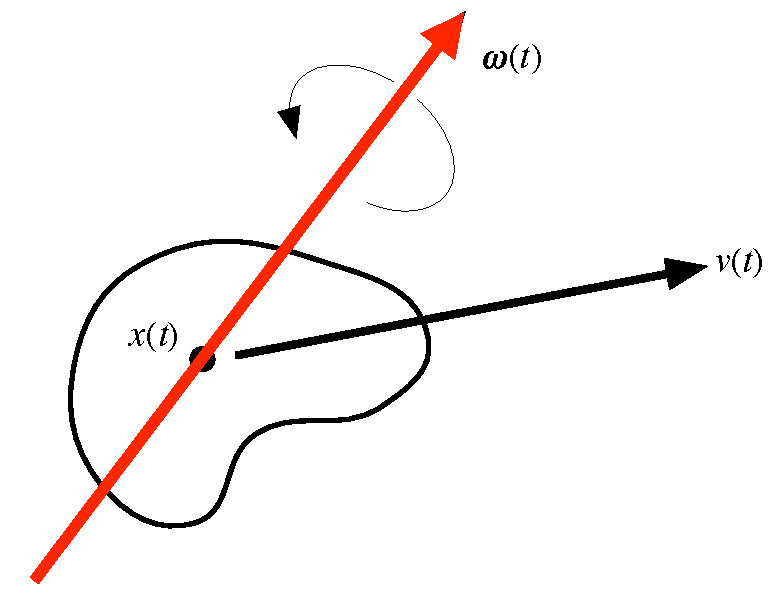
\includegraphics[width=0.45\textwidth]{img/04_spin}
\end{figure}
Where $v(t) = {d\over dt}x(t)$.


\subsection{Total Velocity}
The (constant) location of a particle $i$ in body space is $r_{0_i}$. The location of particle $i$:
\begin{align*}
	r_i(t) = R(t)r_{0_i}
\end{align*}
The velocity of said particle $i$ consists of 
\begin{align*}
\dot r_i &= w(t) \dot R(t) r_{0_i} + v(t)\\
 &= \underbrace{w(t) \times (r_i(t) - x(t))}_\text{angular component} + \underbrace{v(t)}_\text{linear component}
\end{align*}
\begin{figure}[H]
	\centering
	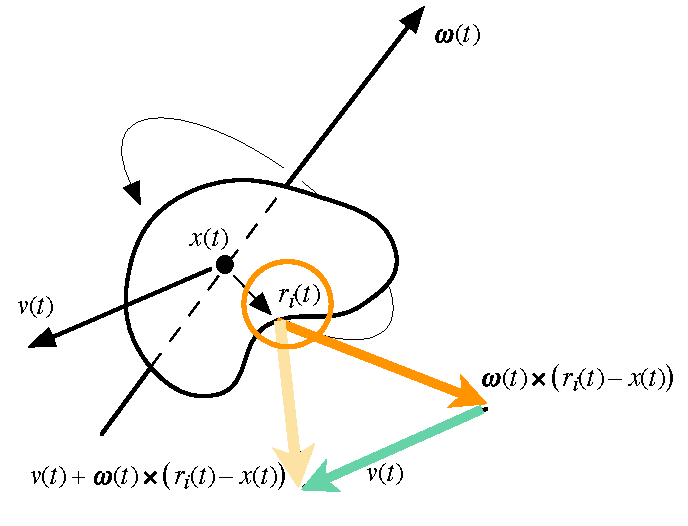
\includegraphics[width=0.45\textwidth]{img/04_total_velocity}
\end{figure}

\section{Rigid Body Dynamics}
\begin{itemize}
	\item External forces (gravity, wind, ...) chaning:
		\begin{itemize}
			\item Linear velocity
			\item Angular velocity
		\end{itemize}
	\item Total force acting on a body
		\begin{align*}
			F(t) = \sum F_i(t) = \sum m_i \dot v_i(t) = M \dot v_{cm}
		\end{align*}
	\item Linear velocity change
		\begin{align*}
			a_{cm} = {F \over M}
		\end{align*}


\end{itemize}



\end{multicols}
